\documentclass[10pt]{article}
\usepackage{icmlko}

\icmlmeta{IP 파운데이션 월드모델}{342}{정보 지도}{계열 넷을 다 섞어 보니 마흔 자리가 갈렸다 --- 그리고 어제 세운 비대칭이 계열 수준에서는 없다}

\begin{document}

\twocolumn[
\icmlheader

\begin{abstract}
노트 341이 검사 ⑤(축이 제 섞은 쌍둥이를 이기나)를 만들어 위키에 돌렸다.
\textbf{나머지 셋에 다 돌렸다} --- 계열 넷 $\times$ 도메인 열 $=$ 마흔 자리.

\begin{center}\footnotesize
\begin{tabular}{lrrl}
\hline
계열 & 검사 ⑤ & 노트 340 ``빼면'' & 이긴 도메인 \\
\hline
\textbf{태그} & \textbf{$+$0.0495} & $-$0.0444 & 웹툰 · 애니 · 세계애니 \\
검색 & $+$0.0395 & $-$0.0343 & \textbf{여덟} \\
달력 & $+$0.0137 & $-$0.0072 & 펀딩 · 웹툰 \\
위키 & $+$0.0024 & $-$0.0070 & 게임 · 세계애니 \\
\hline
\end{tabular}
\end{center}

\textbf{두 자가 같은 순서를 준다} --- 태그 $>$ 검색 $>$ 달력 $>$ 위키가
양쪽에서 같고, 센 둘은 크기까지 가깝다(0.050 대 0.044 · 0.040 대 0.034).
\textbf{어제 세운 ``붙이기와 빼기는 서로의 역이 아니다''가 계열 수준에서는
안 선다.} 노트 341이 본 어긋남은 \emph{제일 약한 계열의 도메인별} 자리였고
거기서는 둘 다 잡음 안이었다. \textbf{고친다.}

\textbf{그리고 계열마다 이기는 곳이 다르다.} 태그는 웹툰에서
$+$0.1615(8/8) --- 마흔 자리 중 제일 크고, 웹툰 큐레이션 태그를 위해
만든 축이다(노트 255). 검색은 도서 $+$0.1195 · 모바일 $+$0.0753 로
\textbf{여덟 도메인에서} 이긴다. 위키는 세계애니 $+$0.0584 하나가 거의
전부다 --- 노트 149가 ``검색 덮음 0\%''를 메우려 만든 바로 그 도메인이다.
\textbf{축은 만들어진 자리에서 값을 한다.}

\textbf{지는 자리도 있다} --- 태그는 아이돌에서 $-$0.0379(2/8), 위키는
시장팝업에서 $-$0.0873(0/8), 검색은 팝업에서 $-$0.0007(4/8).
\textbf{하나도 안 지는 계열은 없다.}
\end{abstract}
]

\section{마흔 자리}

\begin{figure*}[t]
\centering
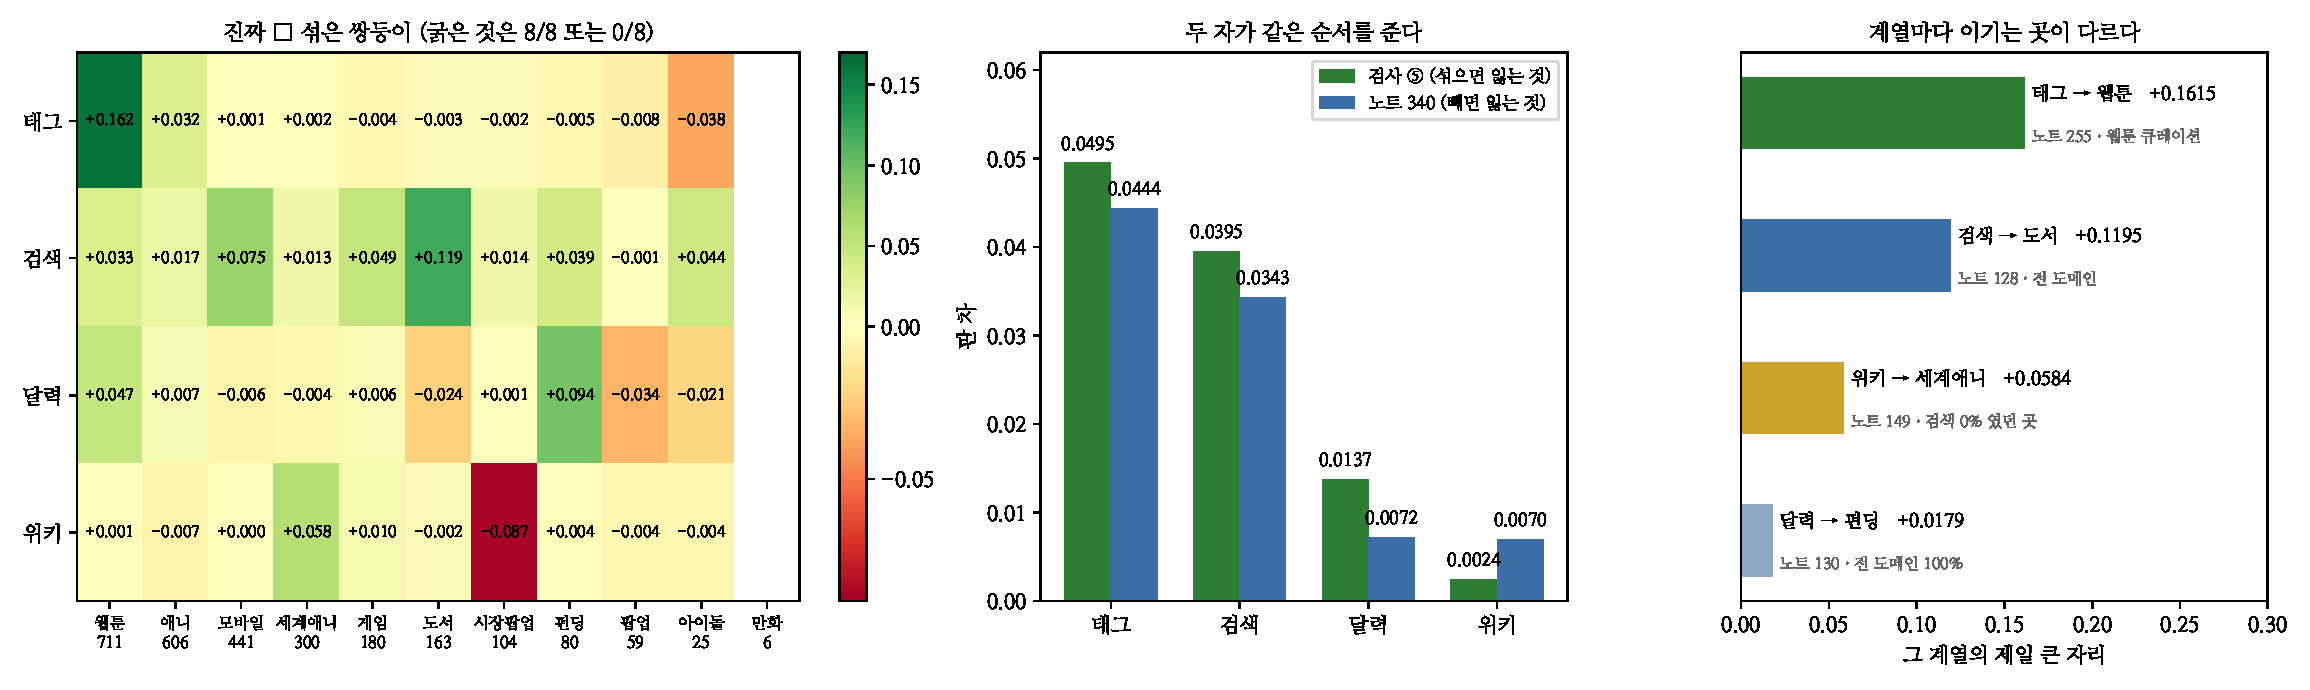
\includegraphics[width=\textwidth]{figs/map.pdf}
\caption{왼쪽 --- 계열$\times$도메인 지도. 가운데 --- 두 자의 순서.
오른쪽 --- 계열마다 제일 큰 자리.}
\end{figure*}

각 자리는 \textbf{그 계열만 섞은 판}과 \textbf{안 섞은 판}을 같은 학습
재추출 뽑기 여덟에서 견준 차다. 양수면 진짜 축이 제 잡음을 이긴다.

\section{어제의 비대칭을 고친다}

노트 341이 ``검사 ⑤ 는 붙일까에 답하지 뺄까에는 답하지 않는다''로 끝났다.
근거는 위키에서 검사 ⑤ 가 시장팝업 $-$0.0873(0/8)이라 했는데 빼 보니
판이 안 움직인 것이었다.

\begin{center}\small
\begin{tabular}{lrr}
\hline
계열 & 검사 ⑤ & $|$빼면$|$ \\
\hline
태그 & 0.0495 & 0.0444 \\
검색 & 0.0395 & 0.0343 \\
달력 & 0.0137 & 0.0072 \\
위키 & 0.0024 & 0.0070 \\
\hline
\multicolumn{3}{l}{순위 상관 \textbf{$+$1.00}} \\
\hline
\end{tabular}
\end{center}

\textbf{계열 수준에서는 두 자가 같다.} 어제 본 어긋남은 \emph{위키 하나}
--- 넷 중 제일 약한 계열이고 두 수(0.0024 · 0.0070)가 둘 다 자기 SD
안이다. \textbf{잡음 안에서 두 자가 다르게 나온 것을 법칙으로 읽었다.}
노트 338이 세운 ``차이도 한 번 재면 안 된다''를 \emph{계열 하나로} 세운
비대칭에도 적용해야 했다.

\paragraph{남는 차이} 센 둘에서 검사 ⑤ 가 ``빼면''보다 0.005$\sim$0.006
크다. \textbf{그것이 잡음 열을 남겨 두는 값이다} --- 섞으면 열이 남아
갈림을 훔치고, 빼면 그냥 없다(노트 340).

\section{계열은 제 고향에서 이긴다}

\begin{center}\footnotesize
\begin{tabular}{llrl}
\hline
계열 & 제일 큰 자리 & 차 & 왜 만들었나 \\
\hline
태그 & 웹툰 & $+$0.1615 & 웹툰 큐레이션(255) \\
검색 & 도서 & $+$0.1195 & 전 도메인(128) \\
위키 & 세계애니 & $+$0.0584 & 검색 0\% 메우기(149) \\
달력 & 펀딩 & $+$0.0179 & 전 도메인 100\%(130) \\
\hline
\end{tabular}
\end{center}

\textbf{태그가 판을 제일 많이 받친다}($+$0.0495)는 것이 뜻밖이다 ---
웹툰 하나를 위해 만든 SVD 축인데, 웹툰이 유보 711행으로 판의 27\%라
그 하나로 판을 끈다. \textbf{그리고 애니에서도 $+$0.0320(8/8) 이긴다}
--- 만들 때 예상 안 한 자리다.

\textbf{검색만 넓다} --- 여덟 도메인에서 이긴다. 나머지 셋은 두셋뿐이다.

\section{지는 자리}

\begin{center}\footnotesize
\begin{tabular}{llrl}
\hline
계열 & 도메인 & 차 & 양수 \\
\hline
위키 & 시장팝업 & $-$0.0873 & 0/8 \\
태그 & 아이돌 & $-$0.0379 & 2/8 \\
태그 & 팝업 & $-$0.0080 & 1/8 \\
위키 & 애니 & $-$0.0070 & 0/8 \\
\hline
\end{tabular}
\end{center}

\textbf{하나도 안 지는 계열이 없다.} 그리고 노트 341이 재 본 대로
\textbf{지는 자리를 빼도 판은 안 오른다} --- 이 지도는 ``어디를 고칠까''가
아니라 \textbf{``이 판의 정보가 어디 있나''}를 말한다.

\section{남은 것}
\begin{center}\footnotesize
\begin{tabular}{ll}
\hline
갈래 & 왜 \\
\hline
\textbf{새 축 후보에 검사 ⑤} & 붙이기 전에 --- 원래 쓰임새 \\
태그를 다른 도메인에 & 애니에서도 이긴다 \\
시장팝업은 왜 다 지나 & 위키 $-$0.087 · 태그 $-$0.002 \\
검색이 왜 팝업만 못 이기나 & 여덟에서 이기고 하나만 진다 \\
\hline
\end{tabular}
\end{center}

\paragraph{규약} \textbf{하나로 세운 법칙은 하나가 무너지면 무너진다.}
어제 위키 한 계열에서 두 자가 어긋난 것을 보고 ``붙이기와 빼기는 서로의
역이 아니다''라는 법칙을 세웠고, 오늘 넷을 다 재니 순위 상관이 $+$1.00
이다. \textbf{n$=$1 로 세운 법칙은 n$=$4 를 못 견딘다.} 노트 324가
``검사 넷이 셋을 갈랐다''를 n$=$3 이라 접었던 것과 같은 자리인데,
\textbf{그때는 스스로 접었고 어제는 안 접었다.}

\end{document}
